\section{Muons}
\label{sec:reco:muon}

\subsection{Muon Inner Detector and Muon Spectrometer Track Reconstruction}
\label{sec:reco:IDMStrk}

\indent Muons are first reconstructed independently in the inner detector (ID) and muon spectrometer (MS). Later information from the ID, MS and calorimeter are combined to form different types of reconstructed muons.  The type of reconstructed muon formed depend on the type of information available.\cite{MuonReco} \\

\indent Muon tracks in the ID are reconstructed using the same algorithm for reconstructing all ID tracks summarized in section \ref{sec:reco:IDtrack}. \\

\indent Muon tracks reconstructed in the MS start by forming segments in each individual muon chamber.  A Hough transform is used to search for hits aligned in the bending $\eta$ plane of the detector.\cite{HoughTrans}  The MDT segments are reconstructed by performing a straight line fit.  The RPC or TGC hits are associated with the MDT segment and measure the coordinate in the non-bending $\phi$ plane.  Segments in the CSC are constructed using a combinatorial search in $\eta$ and $\phi$ planes.  Segment reconstruction require that the segments are loosely compatible with a track originating from the collision point.  \\

\indent Muon spectrometer track candidates are built by fitting together the segments from different muon detector layers.  The algorithm start from seed segments from the middle layer of the MS because the middle layer has more TGC and RPC hits available.  The algorithm searches for other segments in the other layers by matching their relative positions and direction.  Segments are added to the track candidate if they satisfy a set of criteria based on hit multiplicity and fit quality.   Afterwards seed segments from the middle layer have been exhausted, segments in the inner and outer layers are also used as seeds to search for their own tracks.  \\

\indent At least two matching segments are required to build a track, except in the barrel to endcap transition region.  In the transition region, a single high quality segment with both MDT and trigger hits can be considered a track. \\

\indent At this point, the same segment can be in several track candidates.  Overlap removal is then performed to either assign the segment to a single track or allow the segment to be shared between two tracks.  Tracks that share two segments in the inner and middle layer are allowed if there are no shared hits in the outermost layer.  This preserves the high efficiency of reconstructing two close by muons which can result from the two-body-decays of low-mass particles.  \\

\indent Once the track candidate is identified, the hits associated with each track candidate are fitted using a global $\chi^2$ fit.  Hits with large $\chi^2$ are removed and the track is refitted without the outlier hits.  Additional hits consistent with the track trajectory can also be added to the track.  Again the track is refitted if any new hits are added.  A track candidate is accepted if the fitted $\chi^2$ satisfies the selection criteria.  \\

\subsection{Muon Combined Reconstruction}
\label{sec:reco:MuonComb}

\indent Four different types of muons are reconstructed by combining information from the ID, MS, and calorimeters.  The four different types of muons are defined below based on what subdetector information is used to reconstruct them. \\

\begin{itemize}
\item[] {\bf Combined muons:}  Combine muons combine reconstructed ID and MS tracks by performing a global refit that uses all the hits from the ID and MS tracks.  MS hits may be added or removed from the track to improve the fit quality.  The matching between MS and ID tracks are done mostly in an outside-in fashion.  The MS track is extrapolated inwards and matched to an ID track with the energy loss in the calorimeter taken into account.  The inside-out matching approach where the ID track is extrapolated outwards is also used as a complementary method. 
\item[] {\bf Segment tagged muons:}  An ID track is combined with a MS segment in the MDT or CSC to form a segment tagged muon.  The ID track is extrapolated to the MS to find matching segments.  Segment tagged muons add reconstruction efficiency to muons that are either so low $\pt$ that they pass only a single layer of muon detector or are in MS regions with gaps in coverage. 
\item[] {\bf Calorimeter tagged muons (Calo-tagged):}  Calo-tagged muons are built by combining an ID track with calorimeter energy deposits that are consistent with a minimum ionizing particle.  Calo-tagged muons has the lowest purity rate of all reconstructed muons.  However it recovers some efficiency in regions with none or low MS coverage such as the central $|\eta| < 0.1$ region.  The $|\eta| < 0.1$ region is occupied by cabling and servicing to the calorimeter and ID and only has partial MS coverage.  The calo-tagged muon identification algorithm is optimized for the $|\eta| < 0.1$ region and a momentum range of $15 < \pt < 100 \gev$.
\item[] {\bf Extrapolated muons:}  In extrapolated muons the muon trajectory is reconstructed using only the MS track and a loose requirement of compatibility with the interaction point.  Extrapolated muons are used mainly to extend acceptance passed ID coverage in the $2.5 < |\eta| < 2.7$ region.
\end{itemize}

\subsection{Muon Quality}
\label{sec:reco:MuonQuality}

\indent Reconstructed muons are flagged as loose, medium or tight in terms of quality.  The quality selections identify prompt muons originating from the interaction point and reject backgrounds which mainly consist of muons originating from leptonic pion and kaon decays. \\

\indent Pion and kaon decays in-flight can form a muon in the ID that then gets reconstructed as a track in the MS.  The ID track of the muon will have a distinct kink topology. The resulting combined track will have both poor fit quality and poor matching between ID and MS track momenta.  Therefore, combined muon use the following variables to distinguish between high and low quality muons: \\

\begin{itemize}
\item[] {\bf $q/p$ significance:} $q/p$ significance measures the compatibility of the ratio of charge and momentum $(q/p)$ given by the ID and MS tracks. The quantity is normalized to the uncertainty on $(q/p)$ from the two tracks.
\item[] {\bf $\rho\prime$:} $\rho\prime$ is the difference in $\pt$ of the ID and MS tracks divided by the $\pt$ of the combined track
\item[] {\bf fit $\chi^2$:} The $\chi^2$ of the fit to the combined track normalized to the degrees of freedom
\end{itemize}

\indent Quality selections also set requirements on track hits to ensure a robust momentum measurement.  Muon tracks have at least one Pixel hit and at least five SCT hits with fewer than three Pixel or SCT holes.  If the track is located between $\eta$ of 0.1 and 1.9, we also require at least 10 percent of TRT hits originally assigned to the track are still included in the final fit.  \\

\indent Muon quality are split into four categories; {\tt Loose, Medium, Tight,} and {\tt High-$\pt$}.  Loose, medium and tight muons are inclusive of one another.  For example, all tight muons are also included in the looser categories.  Medium muons represent a good balance between momentum resolution and reconstruction efficiency.  Most analysis including this one uses medium muons to identify signal muons.  We use signal muons in multiple one lepton control regions to estimate backgrounds.  We use loose muons to veto on muons in the zero lepton signal and validation regions because of the higher muon reconstruction efficiency. \\

\indent High-$\pt$ muons sacrifices reconstruction efficiency for better momentum resolution in muons with $\pt > 100 \gev$ and are used mainly for heavy resonances searches such as $W\prime$ and $Z\prime$.  We do not use high-$\pt$ muons and will not discuss their identification in detail.  Detailed description of the loose, medium and tight muon categories are given below.  \\

\begin{itemize}
\item[] {\bf Medium muons:} Medium muons are considered the default muons used in physics analysis at ATLAS.  The identification algorithm is designed to minimize systematic uncertainties on momentum measurement and reconstruction efficiency.  Only combined and extrapolated muons are accepted.  Combined muons must have $\ge 3$ hits in at least two separate layers.  The only exception is in the central $|\eta|<0.1$ region where tracks can have at least one MDT layer but no more than one MDT hole is allowed.  Extrapolated muons must have at least three MDT/CSC layers and are allowed only in the forward $2.5 < |\eta| < 2.7$ region which lies outside of ID coverage. $q/p$ significance must be less then 7 in combined muons to ensure good agreement between ID and MS and reject decay-in-flight muons originating from hadrons. 
\item[] {\bf Loose muons:} Loose muons identification is designed to maximize reconstruction efficiency while still ensuring high quality tracks. All combined and extrapolated muons must satisfy the same requirements as the medium muons.  On top of this calo-tagged and segment tagged muons are also allowed in the $|\eta|<0.1$ region in order to increase efficiency.  The majority of loose muons are still combined muons with approximately $97.5\%$ of all loose muons being combined muons in the $|\eta|<2.5$ region.  The rest consist of $1.5\%$ calo-tagged and $1\%$ segment tagged muons.
\item[] {\bf Tight muons:} Tight muons are optimized to maximizes muon purity but costs some reconstruction efficiency.  Only combined muons with hits in at least two muon stations and satisfy the medium definition are accepted.  The combined track fit's normalized $\chi^2$ must also be less then 8.  A two dimensional cut in $\rho\prime$ and $q/p$ significance is also applied.  The 2D cut is tighter for low $\pt$ muons to have better background rejection in a regime where misidentification probability is higher.
\end{itemize}

\subsection{Muon Reconstruction Efficiency and Momentum Calibration}
\label{sec:reco:muonEff}

\indent Muon reconstruction efficiency and muon momenta calibrations are determined by studying narrow resonances decaying into muon pairs in data.  A brief summary is given below and more details can be found in \cite{MuonReco}. \\

\indent Muon reconstruction efficiency is measured in data by using a tag and probe method using $J/\psi\rightarrow \mu\mu$ or $Z\rightarrow\mu\mu$ events.  A well reconstructed muon (medium quality that fires the trigger) is considered the tag.  Then a muon reconstructed using a different system to the one studied for example an bare ID track is considered the probe.  We search to see if the probe is reconstructed as a muon.  We can reject background processes by selecting for events who's tag and probe have an invariant mass and other kinematic features that are consistent with the narrow resonance .  \\

\indent The efficiency for medium and tight muons is a combination of two tag and probe measurements.  First the probability of reconstructing a $X$ muon is tested using a calo-tagged muon as the probe where $X$ is a medium or tight muon.  This essentially measure the probability of identifying a MS track of sufficient quality given an ID track+calo-tagged muon exists.  Then the probability of an ID track of sufficient quality is measured using the MS track as a probe.  The total efficiency is given by equation \ref{eqn:muonEff}. \\

\begin{equation}
\epsilon (X) = \epsilon (X | ID)~\dot~\epsilon(ID) = \epsilon(X | CT)~\dot~\epsilon(ID|MS)
\label{eqn:muonEff}
\end{equation}

\indent We assume that $\epsilon(ID) = \epsilon(ID|MS)$ or that the ID and MS track reconstruction occur independently of one another.  We also assume that the $X$ muon has the same probability of being reconstructed regardless of whether a calo-tagged muon was reconstructed or only an ID track was reconstructed or $\epsilon (X | ID) = \epsilon(X | CT)$. \\

\indent Run 2 muon reconstruction efficiency for loose and mediums are shown in figure \ref{fig:muoneff}. \\

\begin{figure}[htb]
  \begin{center}
    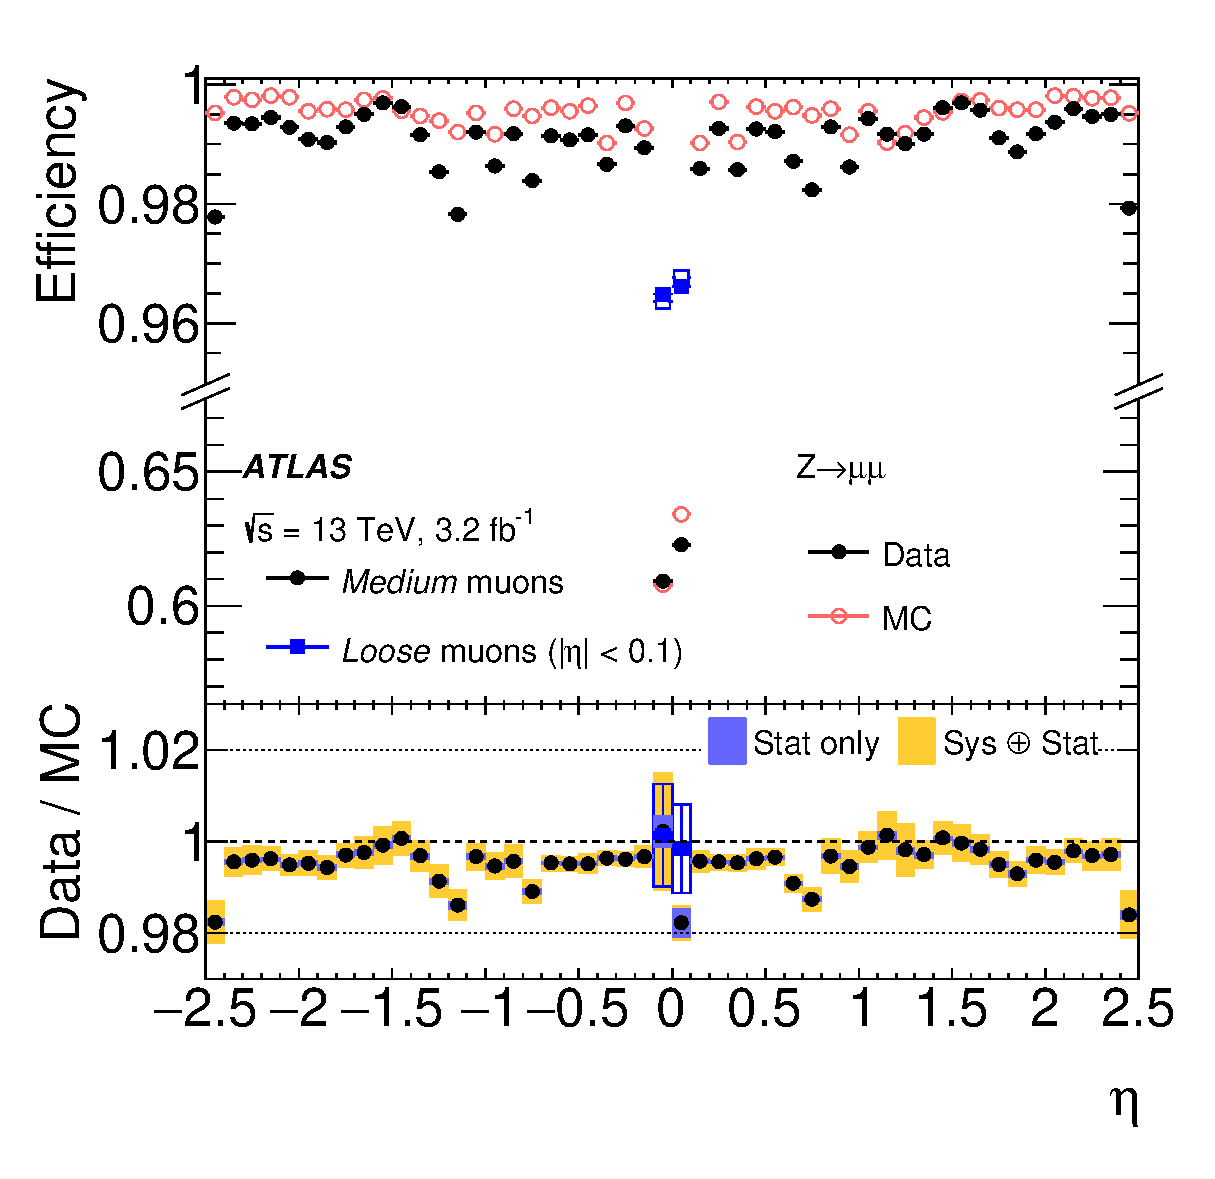
\includegraphics[width=0.55\textwidth]{figures/MuonReco/MuonEff.eps}\hspace{0.05\textwidth}
\end{center}
\caption{Distribution of muon reconstruction efficiency for loose and medium muons.\cite{MuonReco}  Loose and medium muons are identical except in the $|\eta| < 0.1$ region where loose muons also accept calo-tagged and segment tagged muons to recover efficiency.}
\label{fig:muoneff} 
\end{figure}

\indent Muon momentum is calibrated to $J/\psi\rightarrow \mu\mu$ or $Z\rightarrow\mu\mu$ events in data.  The $\pT$ of individual tracks are corrected to account for any inaccuracies in the detector description such as the magnetic field, dimensions of the detector and the amount of energy loss in the calorimeters.  Correction parameters are extracted using a likelihood fit to data with templates derived from MC simulation. MS/ID alignment is also studied using special runs with no magnetic field. The correction parameters differ for different sections of $\eta$ and $\phi$ regions because of the different amount of magnetic fields and independent alignment performed in each section. \\

\indent On top of the total correction to the central value of the $\pt$, the momenta resolution is also estimated using data.  The MC is smeared such that the reconstructed di-muon mass peak agrees between data and MC.  The muon momenta resolution is described according to equation \ref{eqn:muonReso}\\

\begin{equation}
\frac{\sigma(\pt)}{\pt} = r_0/\pt~\oplus~r_1~\oplus~r2~\dot~\pt
\label{eqn:muonReso}
\end{equation}

\indent $r_0/\pt$ accounts for fluctuations in the energy loss in the calorimeter material.  $r_1$ describes multiple scattering, local disturbances in the magnetic field and displacement of hits.  $r2~\dot~\pt$ describes the spacial resolution on the detector hits and any potential mis-alignment in the MS.  Uncertainty on all 3 parameters $r_0$, $r_1$ and $r_2$ are extracted using a likelihood fit to $J/\psi\rightarrow \mu\mu$ or $Z\rightarrow\mu\mu$ events in data. \\

The effect of muon momenta calibration on the MC simulation of $J/\psi\rightarrow \mu\mu$ and $Z\rightarrow\mu\mu$ mass peaks can be seen in figure \ref{fig:muonCalib}. \\

\begin{figure}[htb]
  \begin{center}
    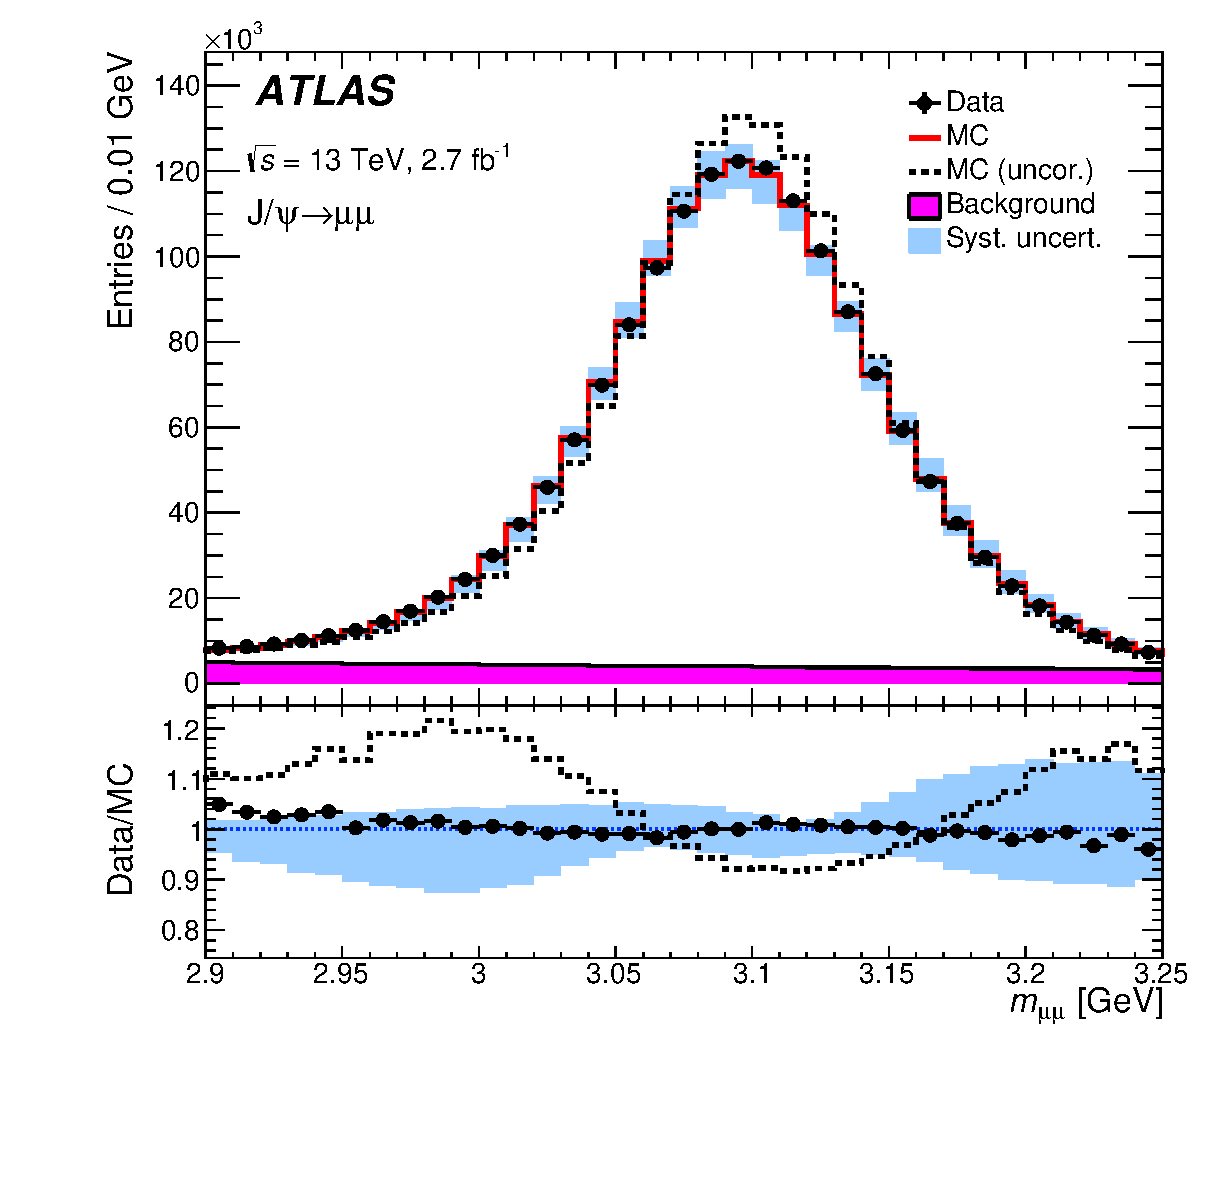
\includegraphics[width=0.45\textwidth]{figures/MuonReco/JPsiMass.eps}\hspace{0.05\textwidth}
    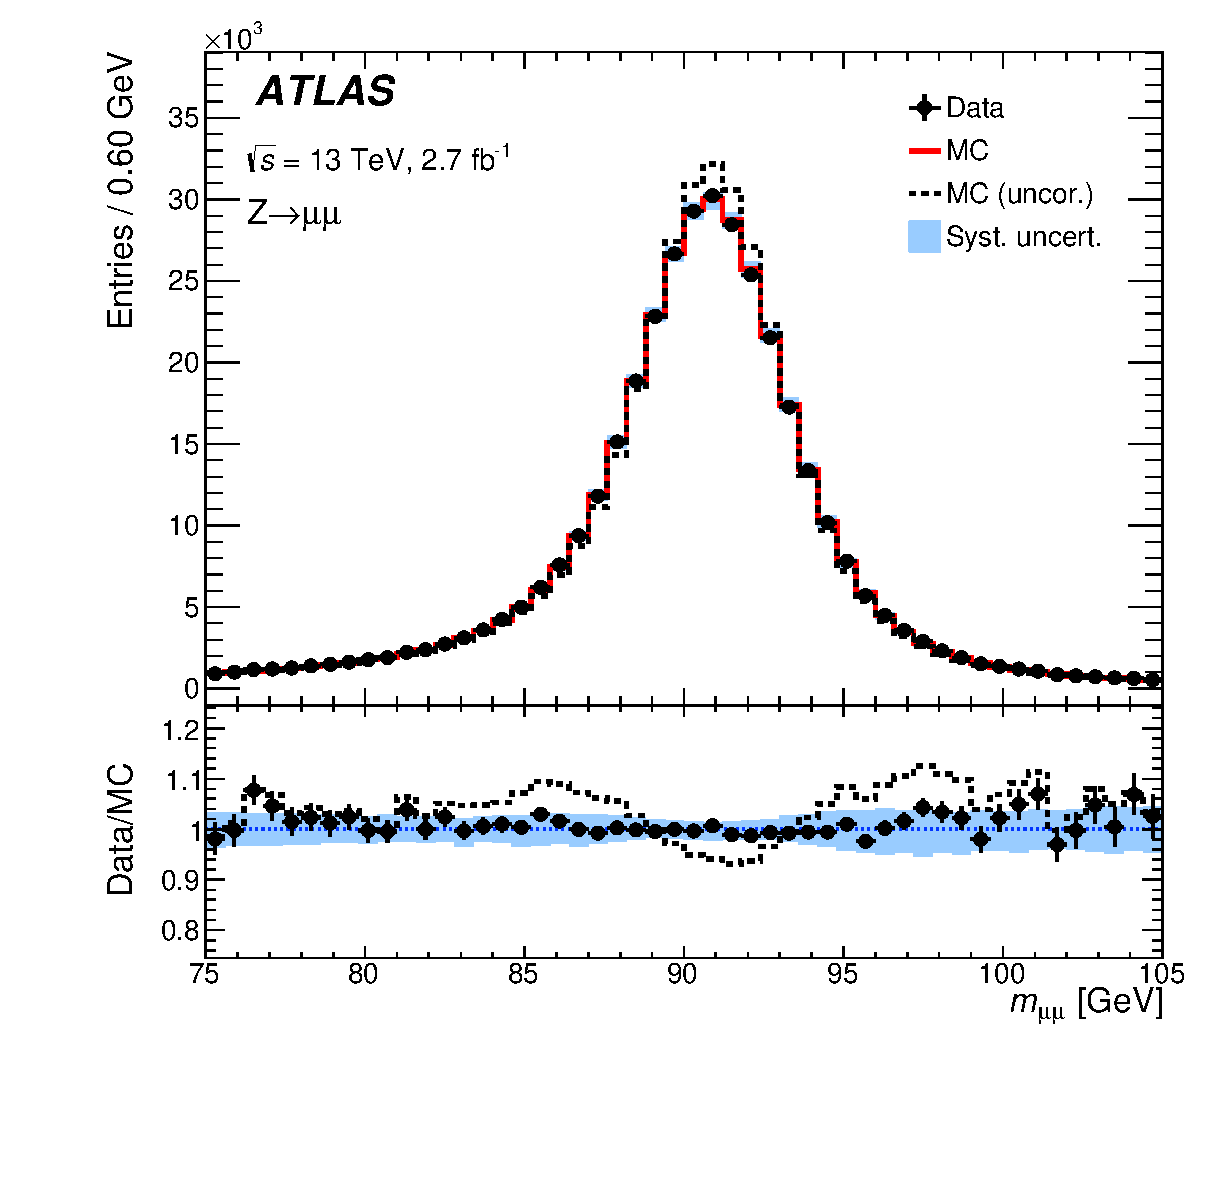
\includegraphics[width=0.45\textwidth]{figures/MuonReco/ZMass.eps}\hspace{0.05\textwidth}
\end{center}
\caption{Dimuon invariant mass before and after muon momenta calibration in data and MC.\cite{MuonReco}}
\label{fig:muonCalib} 
\end{figure}